\chapter{Discussion}

The result shows that FastText can archive better accuracy in general way. We also compare the result between different models.

\section{Discussion}


For the baseline, though TF-IDF it can archive the accuracy about 0.44(±0.04). 
The most distinguishable features they use are some rarely used terminology. 
Since we only removed the duplicated post roughly, it may still suffer from the duplicated post from different sources with certain rarely-used words. 
In general, the model is not general enough, it may not be applicable when the data set changed. 

Additionally, compared to other methods, those approaches convert the sentence to vectors with lower dimensions.
Theoretically, it may benefit the classifier with more dense presentation. Sparse matrix cause much more time and space to train.
With such high dimension vectors, it is unlikely to apply the non-linear classifier.

Generally, FastText can retrieve the better accuracy with segmentation inclusion, and is able to train the large-scale dataset more efficiently with its own classifer.
With conversion to Pinyin, it also achieves the similar accuracy. Though, we tried the different settings for FastText,
the accuracy is not different significantly despite of the various settings of loss function, window size and dimensions. 
In the comparison set, segmented dataset outperforms the one without segmentation. 
It suggested that the term itself may be more meaningful than a single character. And it also took much less time than that of other implementatons.
Although we did not perform it with linear classifier like that in other experiments, we can consider that the accuracy is not lossless.

\section{Baseline}

\begin{CJK}{UTF8}{gbsn}
We used TF-IDF as baseline, the result is 0.44(±0.04), which is statistically greater than the random result in 6 classes problem, 
even we consider the skewed classes.  We tried to evaluate the feature that TF-IDF use to classify as Table \ref{table:featureoftfidf}. 
Though some term here seemed related like, 2nd place in ANGER is \begin{CJK}{UTF8}{bkai}造謠\end{CJK} (create humor),3rd one is 恶浪(violent billow). 
The 2nd place in FEAR is 谋财害命(commit murder for money). The most term is not so related intuitively. 
\end{CJK}

Most of words in each classes actually are not used so commonly. It is contributed by the problem of IDF, which may overweight some rarely-used words.
The other problem is that we observed the netizen keep posting something quite similar like advertisement, joke or news..., 
Though their content are not the same exactly, the words or terminology they used may be quite common. 
Besides TF-IDF, most algorithms assume that the articles themselves are distinct from others. In real world, it is not a common case except some well-organized website articles.
We may require some extra preprocess procedure to handle to prevent intentionally repeated posts.

Some publications\cite{Chen2013TUP25129382512940} shows that the posters may use some morphs to avoid censorship, which we can't evaluate how these words contributes to the sentiment analysis. 
However, the similarity of morphs is quite easy to identified by Word2vec with proper context. 
It is relatively difficult to identify in TF-IDF model. 
\begin{CJK}{UTF8}{gbsn}
\begin{table}[]
\centering
\caption{The feature extracted from TF-IDF}
\label{featureoftfidf}
\begin{tabular}{|c|c|c|c|c|c|}
ANGER	& DISGUST	& FEAR	& JOY	& SAD	& SURPRICE \\
\hline
想瘦	&抬杠	&含铅	&余则	&grunewald	&印钞机 \\
\begin{CJK}{UTF8}{bkai}造謠\end{CJK}	&赃款	&谋财害命	&符离	&节省时间	&绝密\\
恶浪	&由此看来	&表同情	&驻守	&张春桥	&54:03.7\\
顶缸	&淫妇	&经济体	&神明	&前导	&清福\\
银行利息	&\begin{CJK}{UTF8}{bkai}觀天象\end{CJK}	&\begin{CJK}{UTF8}{bkai}可憐見\end{CJK}	&asce	&\begin{CJK}{UTF8}{bkai}已閱\end{CJK}	&任免\\
卫冕冠军	&解除	&突如其来	&三元里	&q1050505041	&karei\\
落水狗	&上刑	&万念俱灰	&何苦来哉	&杀伐	&一桩\\
剖腹自杀	&矢泽爱	&供应站	&太妙了	&离世	&sikucd\\
剥下	&超现实主义	&\begin{CJK}{UTF8}{bkai}勞資\end{CJK}	&两面三刀	&\begin{CJK}{UTF8}{bkai}噴火龍\end{CJK}	&touchsmart610\\
多吉	&\begin{CJK}{UTF8}{bkai}美國使館\end{CJK}	&深红	&slient	&\begin{CJK}{UTF8}{bkai}查無此人\end{CJK}	&翻筋斗
\end{tabular}
\end{table}
\end{CJK}

\section{Siamese-CBOW}

\begin{CJK}{UTF8}{gbsn}
The Siamese-CBOW, the performance is below the baseline. We tried evaluate the model it trained, it seemed it is not converged enough. 
The word embedding is not converted correctly. For example, we use \enquote{我} (I) to query in the word-embedding generated by Siamese-CBOW 5 epoch. 
The related words it show are 扙(hurt, rarely-used word),第四节 (the fourth quarter) and 贾宝玉(the name in the novel). With 10 epoch word embedding, the  
related words are 几家 (Some homes), 峯(peek), and 速成班 (rapid-archieve class). It seemed there is no sign of converge.
\end{CJK}

In the confusion matrix, we found the most tested result fall into two major classes.
It is quite similar as other models due to data imbalance.

We tried to use pre-trained word-embeddings with 10 epoch to improve it, and the result is improved to the level of baseline.
However, when we assessed the embeddings it generated, the embeddings are still far from converging. 
According to original paper, the proper embedding can be trained properly. 
We are not sure if the property is not available in Chinese dataset.

In the original paper, the dataset they conduected is Toronto Books, which contains novels,
 therefore the sematics of the sentences may be more highly coherent with previous sentence and next one. 
The property of the dataset should not affect the word embedding it trains. 
However, it may affect how it determines the relationship between sentences in our cases.

Using some pre-trained embeddings may help to improve the performance. 
Another drawback is that Siamese-CBOW does not support the feature like subword information.
It means if the words is absent from its training dataset, it would be consider non-existent at all. Conducting the vocabulary expansion like that in Skip-Thoughts may assist the problem.


\section{PVDM}

In paragraph vector experiment, the result shows that DBOW produced best accuracy among 3 models. In the original paper, the author suggested that the DM is consistently better than DBOW
, and that the sum version of DM is often better than concatenation. 
So far, it is not clear under what condition that DBOW outperform the DM model. We tried leverge the model it built. 
We fetched most similar word of I (我) as Table \ref{table:doc2vec}. Surprisingly, the similar words of DBOW are all not related words. 
Both DM/C and DM/M generated better results, which top 10 related words are synonyms of I.
It seemed predictable that DBOW stored less data to train. DM/C and DM/M actually model the word in more proper way though the accuracy their accuracy is not good.
Though the result is better for DBOW, it may not be robust result. We need more different datasets to evaluate further.
\begin{CJK}{UTF8}{gbsn}
\begin{table}[]
\centering
\caption{The most similar 5 words of I (我) in 2 models of PVDM}
\label{table:doc2vec}
\begin{tabular}{|c|c|c|c|}
\hline
      & DM/C & DBOW & DM/M \\
\hline
1 & 俺 &  三条  & 偶\\
2 & 偶  & 田徑運動 & 他\\
3 & 老子  & 温暖人间 & 俺\\
4 & 哀家  & youtudou & 我们\\
5 & 皮下  & 化妝水 & 她 \\
\hline
\end{tabular}
\end{table}
\end{CJK}

\begin{table}[]
\centering
\caption{Similar words with \enquote{nǐ}(you) in Pinyin dataset}
\label{table:py_similar}
\begin{tabular}{|c|c|}
\hline
 word related  & Chinese  \\
\hline
wǒ         &   我(I)  \\
nǐzìjǐ     &   你自己(yourself) \\   
nǐmén      &   你們(you)   \\
,"nǐ       &   ,"你(,"you)  \\ 
shuí       &   誰(who)   \\
shuítāmā   &   誰他媽(who in the hell)\\   
wǒhuì      &   我會(I can)   \\
,"shuí     &   ,"誰(who)   \\
,"shuítāmā &   ,"誰他媽(who in the hell)\\   
biérén"    &   別人(others)\\
\hline
\end{tabular}
\end{table}


\section{FastText}

In fasttext, we tried to evaluate the 3 different datasets, segmented, non-segmented and pinyin. 
Although pinyin dataset archieve the same overall accuracy similar to segmented one, the confusion matrix show different tendancy.
Despite of the various settings of loss function, window size, both segmented dataset and non-segmented one classified most entries into 2 major classes.
While with some specific parameters, the classifier on pinyin dataset can classify the minor class as well. 

We tried to validate the property of vectors generated by pinyin dataset with FastText cbow and skip-gram as Table \ref{table:py_similar}. 
It approves that both cbow and skip-gram can generate the pinyin word-embedding efficiently. 
However, for the non-segmented dataset, the word-embeddings consists vectors of single characters, they are not able use subword information neither.

The other finding about word vector it generated. Some segmented dataset contains some poorly segmented term like \enquote{坑爹}(cheating me),\enquote{有木有}(if or not)... 
, which are new internet language so can not be handled properly by dictionary file, are segmented as separate characters.  
While the word2vec can merge those characters together due to the high occurance of these characters. 
Somehow, fasttext treat them as separate term but they may be related highly.

We tried to use T-SNE to visualize the vector space in Figure \ref{tsne}. As we can see, the vector space with some ambiguous boundary.

\begin{figure*}[t!]
    \centering
     
    \begin{subfigure}[t]{0.5\textwidth}
        \centering
        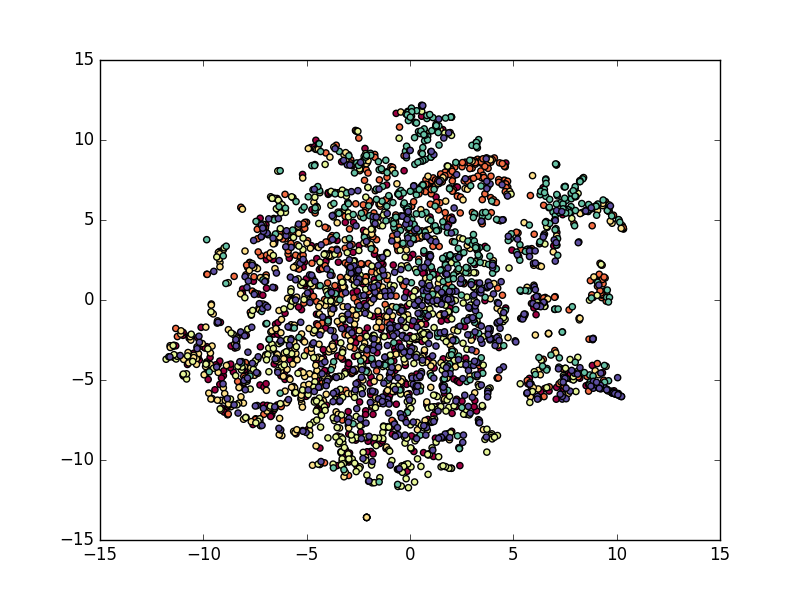
\includegraphics[width=1\linewidth]{ft-All_seg_d200_w15_hs}
        \caption{segmented dataset, dimesion=200 , window size=15, loss function=  hierarchical softmax}
    \end{subfigure}%
    ~
    \begin{subfigure}[t]{0.5\textwidth}
        \centering
        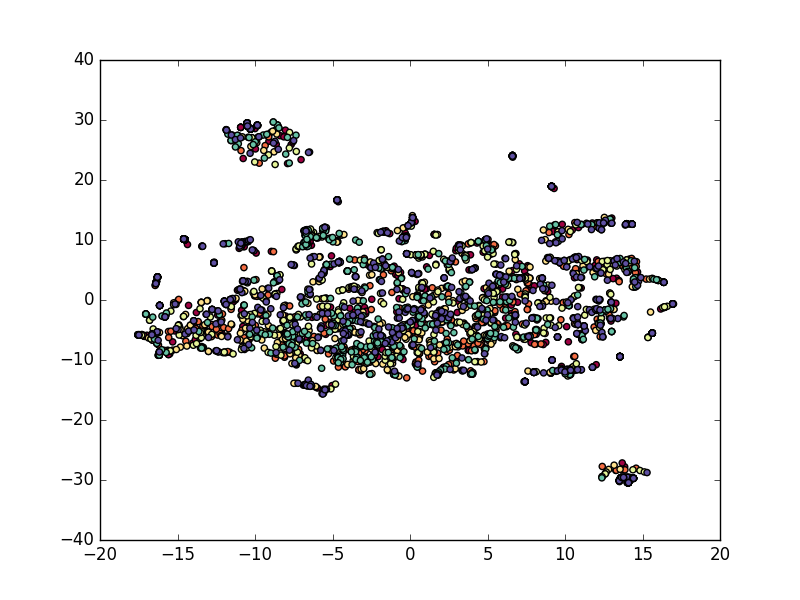
\includegraphics[width=1\linewidth]{fasttext-py-All_seg_d200_w15_softmax_pinyin}
        \caption{pinyin dataset,  dimesion=200 , window size=15, loss function= softmax}
    \end{subfigure}
    \caption{Visualization of vector space for 2 dataset}
    \label{tsne}
\end{figure*}

\begin{CJK}{UTF8}{gbsn}
\begin{table}[]
\centering
\caption{words with low norm in 3 dataset in fasttext}
\label{table:low-norm}
\begin{tabular}{|c|c|}
\hline
 dataset  & words  \\
\hline
segmented  &  旳, 颂, 硬伤, 財, 索取, 图像, 巾 \\
non-segmented  & 喝水还那么麻烦, 给我试试好么@亚瑟小狼狗....etc   \\
pinyin     &         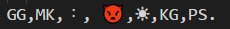
\includegraphics[width=0.5\linewidth]{pinyin} \\   
\hline
\end{tabular}
\end{table}
\end{CJK}

We tried to analyze the vectors it generate. The number of vectors generated with 3 dataset with 100,000 posts are 25,743, 3,137 and 22,233 for segmented, non-segmented and pinyin dataset separately. 
We listed the vectors with lowest norm in Table \cite{table:low-norm}. As the paper indicated that the vector with lower norm, it contains less infomation. 
Therefore, most of them are stop words. Surprisingly, the non-segmented dataset contains much less words than other 2. 
Additionally, the most words it contains are like the sentences rather than the terms. It implied that the fasttext itself can not handle segmentation properly, and explains why it performs poorly. 
For the segmented dataset, the vectors with lowest norm are some rare used words, which can not be modeled properly with low occurance and few neighboring words around.
For the pinyin dataset, the vectors with lowest norm are those special abbreviation and icons. Compared with segmented dataset, those rare used word may have the the same pronunciation with other words or can be inferred from subword information.

%The other property of fasttext is that it is insensitive to sequence of word order in the sentence.

\subsection{N-grams Evaluation}

We evaluated the vectors from ngram level. We found that the term like \enquote{我們}(our) generated by 4 vector: \enquote{我們}, \enquote{\textless 我們}, \enquote{我們\textgreater}, \enquote{\textless 我們\textgreater} in the segmented dataset,
while the counterpart in the pinyin dataset consist 15 vectors, including \enquote{wǒmén}, \enquote{\textless wǒ}, \enquote{\textless wǒm}, \enquote{\textless wǒmé}, \enquote{\textless wǒmén}...etc. 
The segmented n-grams vectors do not contain single character like \enquote{我}, \enquote{們}, becasuse the setting for prefix or subfix for english consist more than 2 or 3 letters above.

We tried to evaluate the word \enquote{我們的}(ours) in both segmented vectors and pinyin vectors in Table \cite{table:ngrams-seg} and Table \cite{table:ngrams-pinyin}. 
We can see the pinyin contain much more conbinations, and the term \enquote{wǒmén-de} which segmented properly indicated high promixity to the complete term. 
In the segmented set, we can see the same tendancy. \enquote{們的}, the term segmented poorly, generate negative similarity. 

The length of ngrams is limited in 3-5 in this experiment. It may be better to model single character in Chinese by shortening the ngram minimum length.
Additionally, the some pinyin may be consituted by only 2 letters.  Lowering the minimum length may model them better as well, but it may also contribute the extra computation effort.
The length of prefix and suffix may vary depending on the languages, so it may be the parameter we can optimize fasttext depends on the language.

\begin{table}[]
\centering
\caption{ngrams constitution of \enquote{我們的}(ours)}
\label{table:ngrams-seg}
\begin{tabular}{|c|c|}
\hline
 key  &  similarity \\
\hline
\textless我們的\textgreater     &  0.02 \\
\textless我們的     &  0.09 \\
我們的\textgreater     &  0.07 \\
們的\textgreater     &  -0.07 \\
我們的     & 0.19   \\
\textless我們     &  *0.99   \\   
\hline
\end{tabular}
\end{table}

\begin{table}[]
\centering
\caption{ngrams constitution of \enquote{wǒménde} (ours) in pinyin}
\label{table:ngrams-pinyin}
\begin{tabular}{|c|c|}
\hline
 key  &  similarity \\
\hline
\textless wǒ -  ménde\textgreater      &  0.73 - 0.14 \\
\textless wǒm -  énde\textgreater      &  0.70 - 0.19 \\
\textless wǒmé - nde\textgreater     &  0.70 - 0.26 \\
\textless wǒmén - de\textgreater      &  0.70 - 0.62\\
wǒmén      &  0.70 \\
  ménde     & 0.16   \\
mén     &  0.35   \\   
\hline
\end{tabular}
\end{table}

\subsection{Subword Information}

According to the paper, the feature subword information can compensate the insufficience of word embeddings. 
We tried to evaluate if the features work in pinyin as well, which means sentimatics can be inferred from the pronunciation. 
Although we converted the dataset to pinyin, the accuracy is not significantly different from the original accuracy. 
Intuitively, pinyin is less readible to native speaker and inreversible to the characters, since the multiple characters own the same pronunciation. 
Chinese contains less syllables and more homonyms than English do. In the original paper\cite{bojanowski2016enriching}, they evaluate the effectiveness in various languages like Arabic, Czech, German, English...etc.
All of them belong to phonography, and most languages belong to phonography. While Chinese belongs to logogram specially. 

We tried some examples in segmented and pinyin dataset in Table \cite{table:related-words}
The term acquired shared some similarity in consitute characters, and their meaning are similar by some degree.
In the example of pinyin seemed only return the terms with morphological similarity.
So far, we are still hard to quantize the effectiveness conducted in Chinese.

In the \cite{DBLP:journals/corr/MikolovLS13}, it provides similar function to compensate the words absent from training set. 
It employs similarity of pre-trained word-embedding, rather than the similarity of n-gram characters features. 
There are also some differnet approaches like morphologically annotated data, whcih were introduced by Cotterell and Schütze (2015).
It may be a good topic to evaluate the difference of these approaches. 

\begin{CJK}{UTF8}{gbsn}
\begin{table}[]
\centering
\caption{Query the word non-existing in dataset}
\label{table:related-words}
\begin{tabular}{|c|c|c|}
\hline
 吃不起 & 给力 & gōngxǐfācái(恭喜發財)  \\
\hline
吃不饱  & ok & gōngxǐ (恭喜)\\
买不起  & 得意 & gōngqíjùn (宫崎骏)\\
吃不完     &  [ & gōngpū(公布)\\   
上不起     &   lt & gōngrè(公认) \\   
经不起     &   想念 & gōngpó(公婆)\\
\hline
\end{tabular}
\end{table}
\end{CJK}

\section{Conclusion}

We demonstrated the various modern methods on the Chinese corpus, and it indicated that some models like FastText are invariant to language property. 
In general, most models improve the sematic analysis compared with tranditional TFIDF, and it is more efficient to extract the informance with more dense vectors.

Most methods are developed with English property, so segmentation plays a crucial role to make the Chinese posts look like English.
 But the segmentation may also contribute something wrong. Though FastText also can be conducted with non-segmented sentences, it performed worse due to improper segmentation.

We can see fasttext demostrate excellent property in both performance including training and testing time and memory utilization. 
Besides the accuracy of the sematic conversion, both the performance and the efficiency of memory also become the interest of study.

